\let\negmedspace\undefined
\let\negthickspace\undefined
\documentclass[journal]{IEEEtran}
\usepackage[a5paper, margin=10mm, onecolumn]{geometry}
%\usepackage{lmodern} % Ensure lmodern is loaded for pdflatex
\usepackage{tfrupee} % Include tfrupee package

\setlength{\headheight}{1cm} % Set the height of the header box
\setlength{\headsep}{0mm}     % Set the distance between the header box and the top of the text

\usepackage{gvv-book}
\usepackage{gvv}
\usepackage{cite}
\usepackage{amsmath,amssymb,amsfonts,amsthm}
\usepackage{algorithmic}
\usepackage{graphicx}
\usepackage{textcomp}
\usepackage{xcolor}
\usepackage{txfonts}
\usepackage{listings}
\usepackage{enumitem}
\usepackage{mathtools}
\usepackage{gensymb}
\usepackage{comment}
\usepackage[breaklinks=true]{hyperref}
\usepackage{tkz-euclide} 
\usepackage{listings}
% \usepackage{gvv}                                        
\def\inputGnumericTable{}                                 
\usepackage[latin1]{inputenc}                                
\usepackage{color}                                            
\usepackage{array}                                            
\usepackage{longtable}                                       
\usepackage{calc}                                             
\usepackage{multirow}                                         
\usepackage{hhline}                                           
\usepackage{ifthen}                                           
\usepackage{lscape}
\begin{document}

\bibliographystyle{IEEEtran}
\vspace{3cm}

\title{NCERT-6.5.14}
\author{EE24BTECH11065 - Spoorthi yellamanchali
}
% \maketitle
% \newpage
% \bigskip
{\let\newpage\relax\maketitle}

\renewcommand{\thefigure}{\theenumi}
\renewcommand{\thetable}{\theenumi}
\setlength{\intextsep}{10pt} % Space between text and floats


\numberwithin{equation}{enumi}
\numberwithin{figure}{enumi}
\renewcommand{\thetable}{\theenumi}


\textbf{Question:}
\\
Find two positive numbers $x$ and $y$ such that $x + y$ = 60 and $xy^3$ is maximum.
\\
\textbf{ Theoretical Solution: }
\\
From the question, we can write,
\begin{align}
        y = 60 - x
\end{align}
On substituting equation $\brak{0.1}$ in $xy^3$, we get,
\begin{align}
    x\brak{60 - x}^3
\end{align}
On differentiating equation $\brak{0.2}$ with respect to $x$ and equating it to zero, we get,
\begin{align}
    \brak{60 - x}^3 - 3x\brak{60 - x}^2 = 0\\
    \brak{60 - x}^2\brak{60 - 4x} = 0
\end{align}
From the equation $\brak{asd}$, we get , $x = 60$ and $x = 15$,\\
On differentiating equation $\brak{asd}$, with respect $x$, and substituting both values of $x$, we get,
\begin{align}
    -3\brak{60 - x}^2 -3\brak{60 - x}^2 + 6x\brak{60 - x}\\
    \therefore \frac{d^2y}{dx^2} = \brak{60 - x}\brak{-360 + 12x}
\end{align}
On substituting $x = 15$, we get ,
\begin{align}
    \frac{d^2y}{dx^2} < 0 
\end{align}
that means, $xy^3$ is maximum when $x = 15$, then , $y = 60 - 15=45$\\
$\therefore$ $xy^3$ is maximum when $x = 15$ and $ y = 45$.\\
\textbf{Solution using gradient descent method.}
\\
The gradient descent(in case of finding minima) or the gradient ascent method(in case of finding maxima) is a computational algorithm which optimizes and maximises/minimizes the functional curve.\\
It uses the concept of gradient or slope to do so as we know the fact that slope or gradient is zero or almost negligible at points of maxima and minima.\\
It works by itertively adjusting the input variable $x$ in the direction of function's gradient.\\
starting from initial guess $x_0$,the algorithm iteratively updates $x$ using the rule\\

\begin{align}
    x_{new} = x_{current} + \alpha \times f^\prime\brak{x_{current}}
\end{align}

Here $\alpha$ is the learning rate which controls the size of each step.\\
The iteration stops when the change in $x$ between iterations becomes smaller than a predefined tolerance.\\
We know that, in our question,
\begin{align}
    f^\prime \brak{x} = -3x\brak{60-x}^2 + \brak{60-x}^3
\end{align}
On substituing equation $\brak{0.9}$ in $\brak{0.8}$ , we get,
\begin{align}
    x_{new} = x_{current} + \alpha\brak{-3x_{current}\brak{60-x_{current}}^2 + \brak{60-x_{current}}^3}
\end{align}
and by taking,
\begin{align}
    \alpha = 0.000001\\
\end{align}
And convergence = $1e-6$\\
initial guess $x_0$ = 14.0,
We get,\\
$x$ value at maxima =  14.999878397267214\\
$y$ value at maxima =  1366874.999940112\\

\begin{figure}[h!]
   \centering
   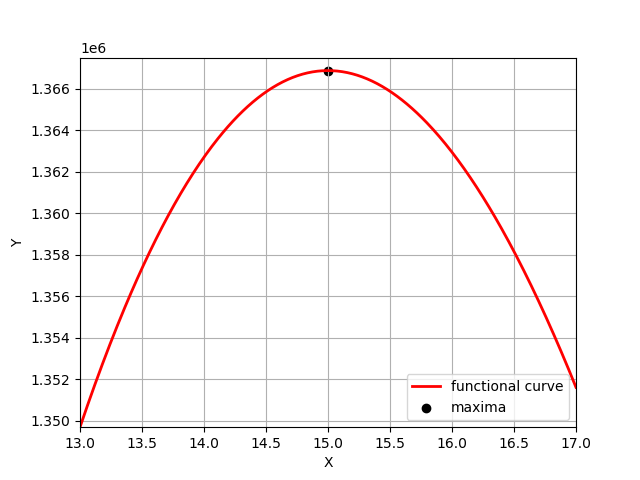
\includegraphics[width=0.75\columnwidth]{figures/Figure_1.png}
   \label{graph of the function}
\end{figure}

\end{document}


